 % last updated in April 2002 by Antje Endemann
% Based on CVPR 07 and LNCS, with modifications by DAF, AZ and elle, 2008 and AA, 2010, and CC, 2011; TT, 2014; AAS, 2016

\documentclass[runningheads]{llncs}
\usepackage{graphicx}
\usepackage{amsmath,amssymb} % define this before the line numbering.
\usepackage{ruler}
\usepackage{color}
\usepackage[width=122mm,left=12mm,paperwidth=146mm,height=193mm,top=12mm,paperheight=217mm]{geometry}
\usepackage{appendix}
\usepackage{hyperref}
\usepackage{subfigure}
\usepackage{graphicx, subcaption}
\usepackage{comment}

\begin{document}
% \renewcommand\thelinenumber{\color[rgb]{0.2,0.5,0.8}\normalfont\sffamily\scriptsize\arabic{linenumber}\color[rgb]{0,0,0}}
% \renewcommand\makeLineNumber {\hss\thelinenumber\ \hspace{6mm} \rlap{\hskip\textwidth\ \hspace{6.5mm}\thelinenumber}}
% \linenumbers
\pagestyle{headings}
\mainmatter
\def\ECCV18SubNumber{***}  % Insert your submission number here

\title{Denoising 3D Time-Of-Flight Data} % Replace with your title

\titlerunning{ECCV-19 \ECCV18SubNumber}

\authorrunning{ECCV-19 \ECCV18SubNumber}

\author{Kapil Gupta, Yanwen Xu}
\institute{University of California, Santa Cruz}


\maketitle

\begin{figure}
    \centering
    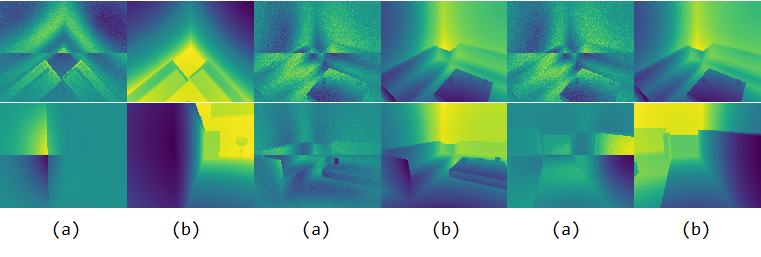
\includegraphics[scale=0.6]{img/depthmap/Figure_1.png}
    \caption{
    From (a) noisy depth images corrupted by Multi-path Interference  to (b) highly-accurate depth images, our two-part CNN model can efficiently and robustly remove artifacts in synthesized Time-of-Flight camera images. }
    \label{fig:result_raw}
\end{figure}

\begin{abstract}
Depth Perception is widely used in several computer vision tasks. The most common method for depth calculation is range imaging cameras such as Time of Flight (ToF) cameras.  However, ToF cameras suffer from non-negligible noise caused by Multi-Path Interference (MPI). While various classical methods exist, machine learning techniques have not been explored as much due to the lack of ground-truth data. In this paper, we propose a novel method for MPI noise removal using a two-part convolutional neural network. The first model learns about the core properties of the reflective objects in the scene, such as the reflectively of the scene and local ambient light density.  The second model learns to map such properties along with a False Depth Map to create a True Depth Map of the scene. We demonstrate and validate our results on a synthetic dataset. The source code for this work is present at \href{https://github.com/daemonslayer/3d-tof-denoising.git}{\textbf{github.com/daemonslayer/3d-tof-denoising}}

\keywords{time-of-flight, multi-path interference, deep learning}
\end{abstract}


\section{Introduction}
% -----------------------------------------------------------------------------------------------

3D imaging systems provide depth information that is crucial in a diverse range of computer vision applications. Depth Sensors using Time-of-Flight(ToF) imaging are the most popular amongst such cameras due to cheap cost. Range Imaging and Depth Perception that is available from such cameras can be used for several computer vision tasks such as gesture recognition, image quality improvement, and obstacle avoidance. 
Nevertheless, ToF cameras suffer from various sources of noise caused by the following: the presence of ambient light, the interference due to different modulating frequencies, the noise caused by multiple reflections, the motion introduced by the subject, and the shot noise by the camera's electronics. 
In this paper, we focus on the noise caused due to multiple reflections that makes accurate depth calculations difficult. 
\newline
\newline
3D ToF cameras send a pulsed ray of light and record the time taken for the light ray to reach the sensor. The time taken and the phase shift between the original and reflected wave can be used to calculate the distance of an object in the scene from the camera. The camera's depth map acquisition is based upon the assumption that the ray of light is reflected only once in the given scene before reaching the sensor. However, objects with different specularity can scatter light differently, causing multiple reflections with different objects present in the scene. The delay caused by multiple reflections causes an error in the depth calculation. This is an inherently hard problem because the level of MPI error depends on the properties of objects in the scene, as well as the ambient lighting of the scene. 
\newline
\newline
% Talks about previous works
% 
Previous solutions \cite{tomasi1998bilateral,zhang2014rolling} to this issue are performing traditional approaches such as Bilateral filtering on the depth image. 
Bilateral filtering is suitable for Photon Shot Noises because of its nature of taking the average intensity of nearby pixels. 
However, traditional approaches are not necessarily optimal for MPI noises because of its complexity. 
Particularly for MPI denoising, attempts have been made, such as modifying the reflection to get away with errors. 
However, this approach is neither generic nor practical in real-world applications. 
Convolutional Neural Networks (CNN) were commonly used in image denoising. 
Other data-driven approaches \cite{bolsee2018cnn,marco2017deeptof} takes advantage of machine learning, which is to train deep neural networks with synthetic data generated by ToF simulators. 
While the network can somewhat reduce artifacts, it does not entirely remove them. 
Moreover, it still reminds uncertain that if the model trained from synthetic data would apply to real-world data. 
\newline
\newline
We propose a novel method for removing noise caused due to Multi-Path Interference. We use a two-part Convolutional Neural Network that is trained on synthetic data. The first CNN is used to learn the essential properties of the scene, such as the specularity of objects present in the scene, ambient light, and camera position. The second CNN takes the given parameter values from the first model, along with a noisy depth map to generate the true depth map. Our method is based on the observation that MPI noise is directly dependent upon properties of the scene, and hence learning those properties can help determine the depth map with accurate depth information. To our knowledge, such two-part strategy has not been used before in the MPI-denoising context. 
\newline
\newline
We describe our contribution as following: 
\begin{enumerate}
    \item A two-stage training strategy, which first extracts important scene parameters from a noisy depth map and then uses those parameters along with a noisy depth map to create a highly-accurate depth map.  
    \item A practical trained network that removes MPI noise from a single ToF image in real-time and outperforms the state-of-art methods.
    \item A method that is able to process highly specular objects in a scene that may introduce high MPI noise.
\end{enumerate}


\section{Related Work}

\subsection{Classical approaches} MPI Error is caused due to multiple photon intersections, leading to an error in measurements. 
If multiple modulation frequencies of light are used, the time delay operator can be used to process the measurements in the Fourier domain\cite{bhandari2016}. 
In a controlled setting, 2K+1 measurements are needed to recover depth information from K interfering rays of light\cite{bhandari2015}. 
Local and global illumination information has also been used along with the depth information recovered by the ToF camera to overcome MPI based noise\cite{naik2015}.
Light Transport methods that are based on the idea that direct light follows the epipolar line and indirect light does not have been successfully used to remove indirect light from the scene\cite{otoole2014}. 
Further work has been done in separating various transformations indirect light caused by the path of light in the scene in the temporal domain\cite{otoole2014siggraph}
For several other interesting approaches to MPI based noise correction, the reader should refer to the survey paper by Whyte et al. \cite{whyte2014}
.

\subsection{Learning based Methods}
Due to substantial data requirements for this approach, and lack of available datasets with high-quality ground-truth, Deep Learning approach has not been widely used yet. 
Qi et al. used the Transient Rendering method to generate scenes with varying specular properties and ambient lighting conditions. Along with a simulator for introducing noise into the scenes, Qi et al. created a pipeline method \cite{guo2018flat} to correct various noises simulated by the dataset, including shot noise, multi-path inference noise, noise introduced by dynamic scenes.  
A two-network ad-hoc method for depth refinement has been used, where a coarse network first learns the global structure, and then another network attempts to remove MPI noise while preserving details.
GAN\cite{agresti2019unsupervised} was used to perform domain adaptation from synthetic data to real data after learning to remove MPI noise using a CNN based model. A self-supervised method \cite{sterzentsenko2019} that uses deep autoencoder along with geometric priors taken from differentiable rendering was also used to remove MPI error. 
\newline
\newline
Even though there have been several papers using synthetic data, the performance on the real-world dataset has not been that great. 
This is possible because the statistical patterns of noise seen in real-world data cannot be patterned well by the synthetic dataset.




% ========================================================================================
% Data Section
% ========================================================================================

\section{Dataset} 

\begin{figure}
    \centering
    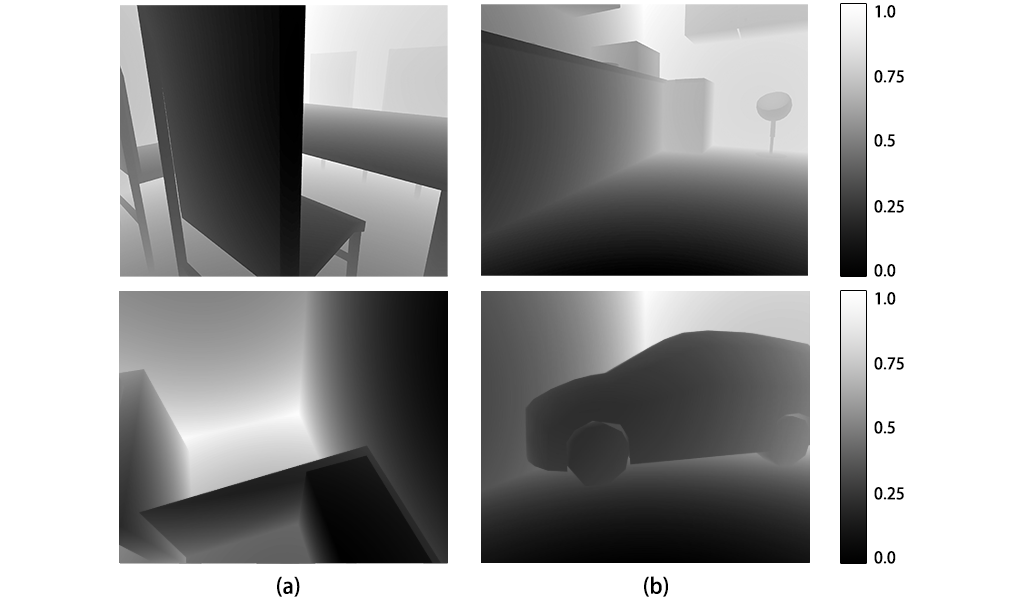
\includegraphics[scale=0.35]{img/depthmap/raw.png}
    \caption{Transient Rendered Scene}
    \label{fig:result_raw}
\end{figure}

We used Nvidia's synthetic data for the initial training of our deep learning model. We captured 30 images from different positions of more than 900 different scenes with reflective objects placed in various positions in a room. The scenes were first rendered using transient rendering method\cite{jarabo2014} using the same camera FOV as Kinect. The noise was then introduced to these scenes using FLAT's Kinect sensor model. The model is trained on Kinect data and hence understands the statistical properties of noise from the sensor. We collected 100 images from 20 different scenes using a Canesta D350 3D Time-of-Flight camera.  All scenes had objects with varied specular properties, thus introducing MPI with the varying amount. The ambient light was not controlled, providing very close to real-world conditions.


% -----------------------------------------------------------------------
% Proposed method
% -----------------------------------------------------------------------

\section{Proposed Method}

\begin{figure}
    \centering
    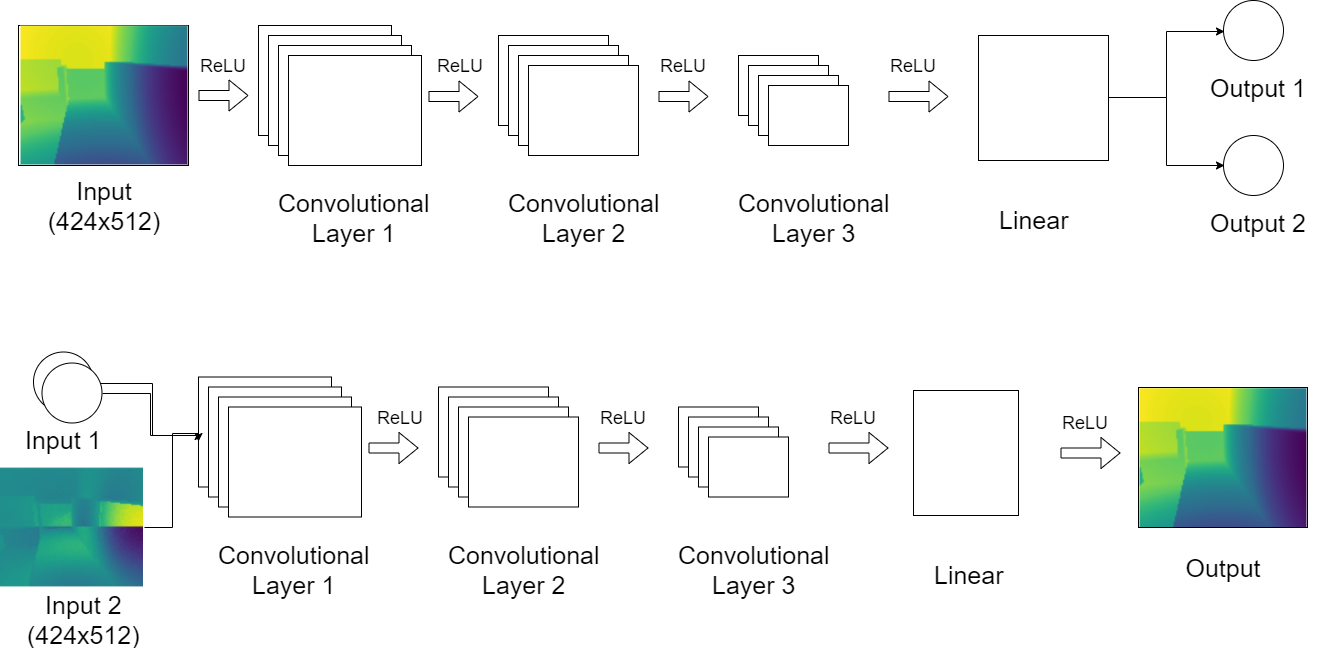
\includegraphics[scale=0.25]{img/NN-model/CNN2.png}
    \caption{Proposed CNN architecture. The first model takes the false depth map of shape (424x512) as input, and outputs the light positions in the scene, lambertian reflectance values of objects in the scene and position of camera relative to scene origin. The second model takes as input the false depth map (424x512) as well as the output values of first model(18x1) and provides the accuracte depth map as output(424x512). }
    \label{fig:result_raw}
\end{figure}

We propose a two-part convolutional neural network model to eliminate MPI noise from images captured using a Time-of-flight camera. 
We demonstrate the use of this model on synthetic data created using the FLAT dataset by Nvidia, which generates Kinect camera-based data. 
\newline
\newline
The first CNN is used to predict scene parameters from a noisy depth map input. The scene parameters include position of lights in the scene, lambertian reflectanct of objects in the scene and the camera position with respect to origin. The ground-truth parameters are available in the synthetic dataset. The first CNN outputs the correct parameters as an (18x1) vector. The input shape of the image is (424x512), and the output values are (18x1) vectors. The scene parameters along with the noisy depth map are used as input for the second CNN. The second CNN model outputs the (424x512) with the corrected depth map.
\newline For the first model, we used five Convolutional layers with a kernel size of 5, a stride value of 1, and a padding value of 2. The output channels were [16, 32, 64, 32, 16] respectively. The convolutional layers were followed by a linear layer that provides vector outputs.
\newline
For the second model, we used five convolutional layers with a kernel size of 5, a stride value of 2, and a padding value of 2. The output channels were [16, 32, 32, 32, 16, 1]. The parameter vector from first model was input into a convolutional layer with kernel size of 5, stride of 2 and 32 output channels. This layer was then concatenated with the output of layer 3 in order to use the scene parameters while predicting the correct depth map.
Using such a two-part model gives better control over the training, and provides the model with more information to create accurate depth maps. We initially used Mean Squared Error Loss for the first model. During fine-tuning the model, the error value from reconstruction of true depth map was also added to the MSE Loss. For the second network, we used per-pixel squared difference as the loss function. We used a Nvidia Tesla V100 with 32GB of GPU memory and a 42 core Intel CPU for parsing throught the dataset.


% -----------------------------------------------------------------------
% Evaluation
% -----------------------------------------------------------------------

\section{Experiments}

In our model, we needed to concatenate the scene parameter vector to the second model in order to train the network to learn true (denoised) depth maps. We experimented with multiple methods of doing do, such as upsampling the parameters using a Fully Convolutional Network and increasing the number of channels by padding the vector to same channels as the second network's layer. We also tried upsampling the parameter vector using Transposed Convolution Layer in pytorch and then appending this new vector to the network.

Finally, we decided to append the parameters as extra channels along with the channels from the third layer in the network. 

\section{Evaluation}

\begin{figure}
    \centering
    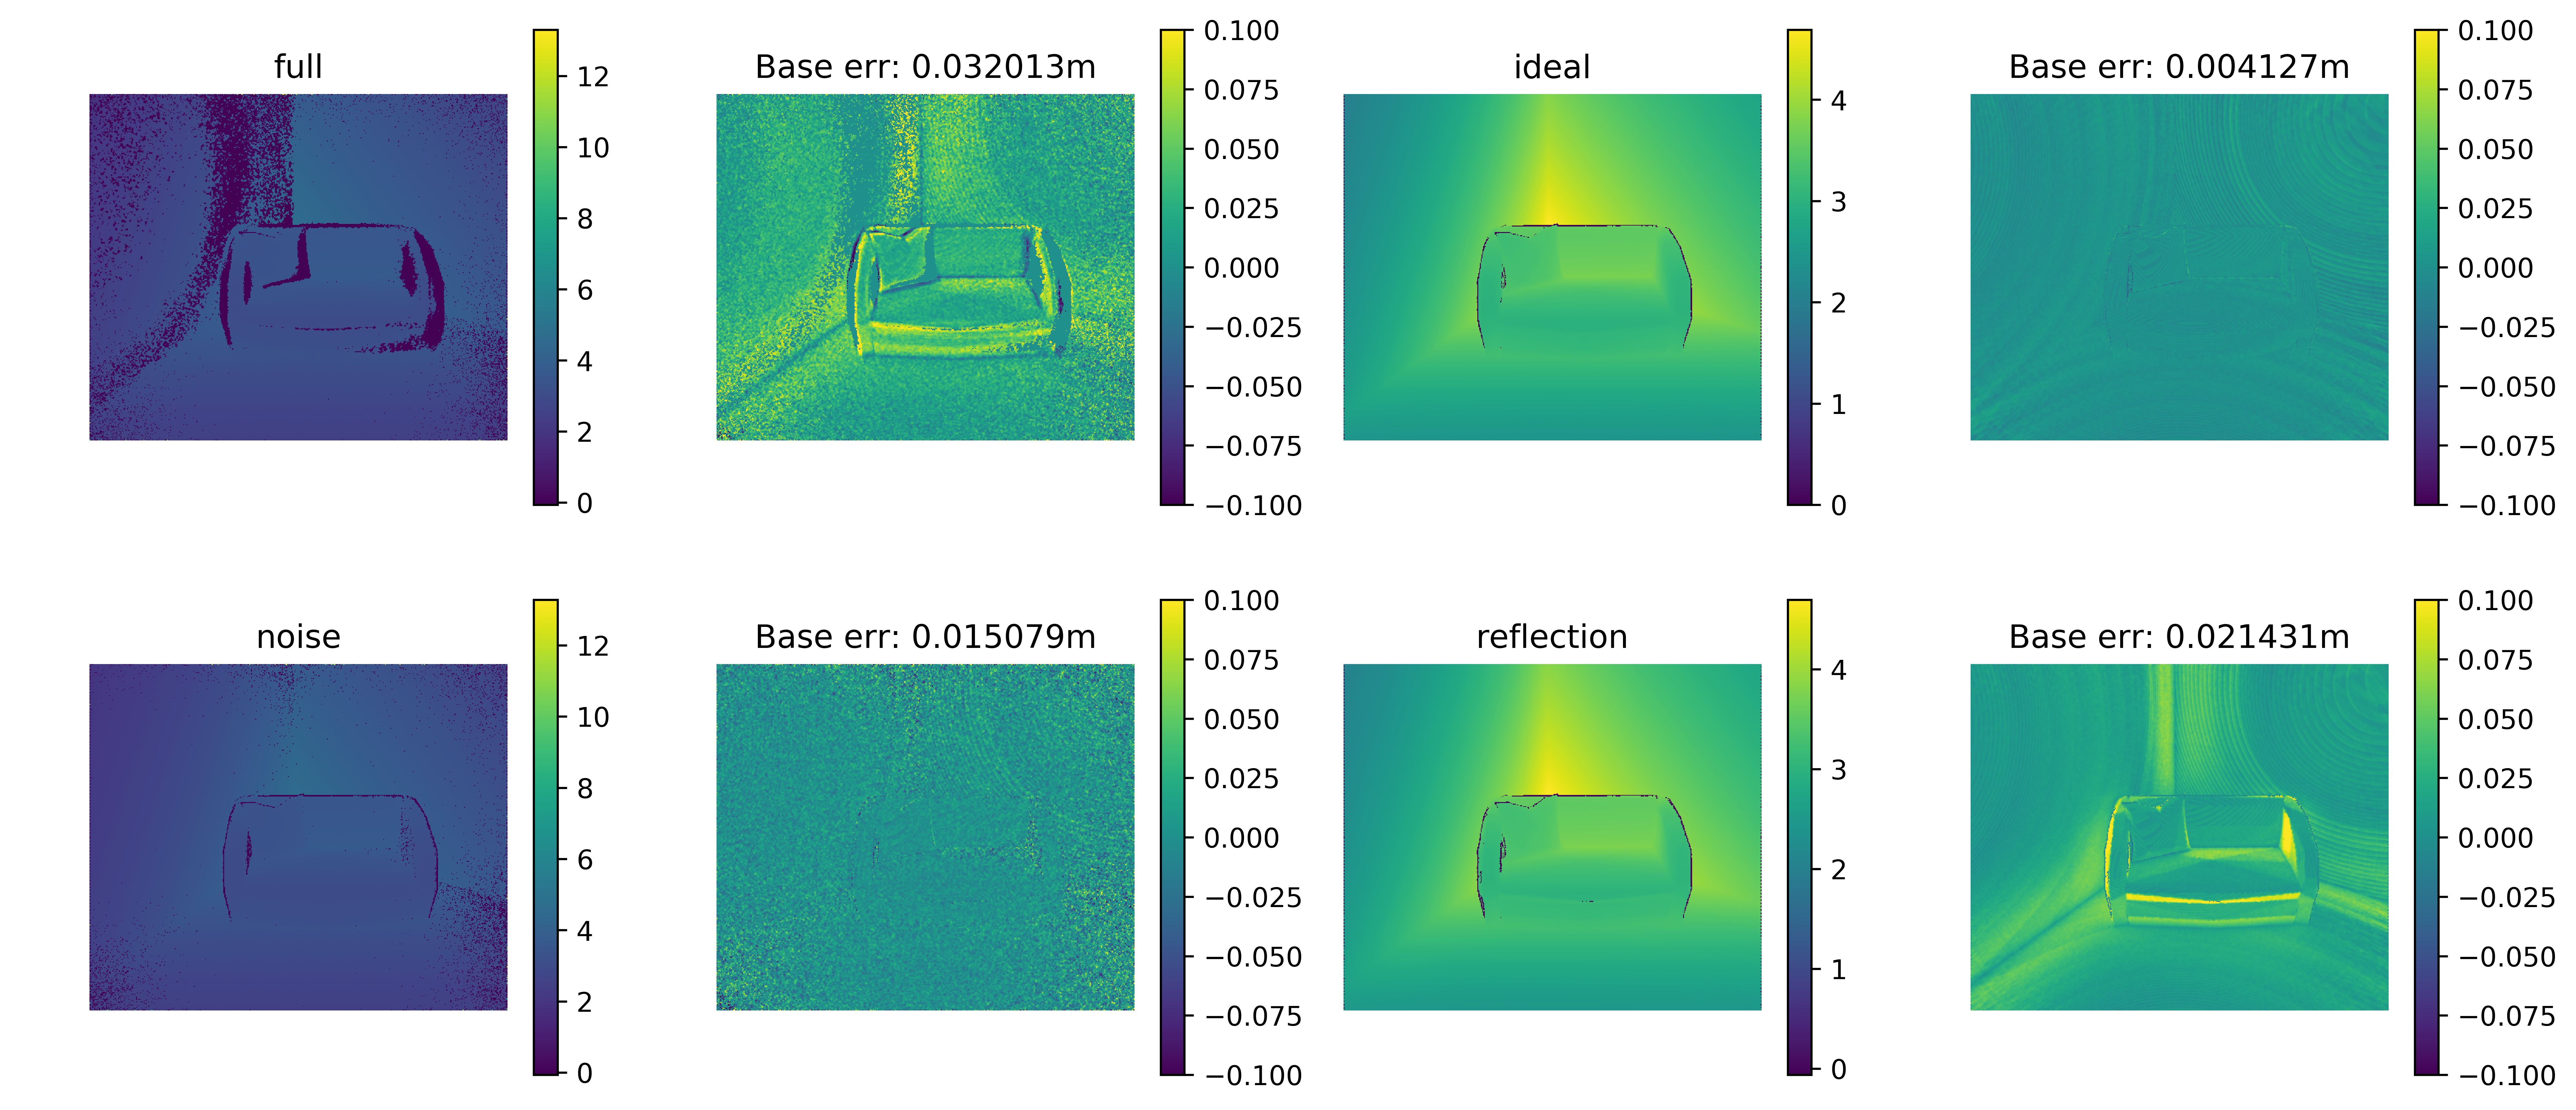
\includegraphics[scale=0.35]{img/depthmap/error.png}
    \caption{Error introduced in ideal images using Kinect mask. Possible noises can be all possible noises(full), sensor noise(noise) and MPI based noise(reflection). }
    \label{fig:result_raw}
\end{figure}

\begin{comment}
\begin{figure}
    \centering
    
    \subfigure{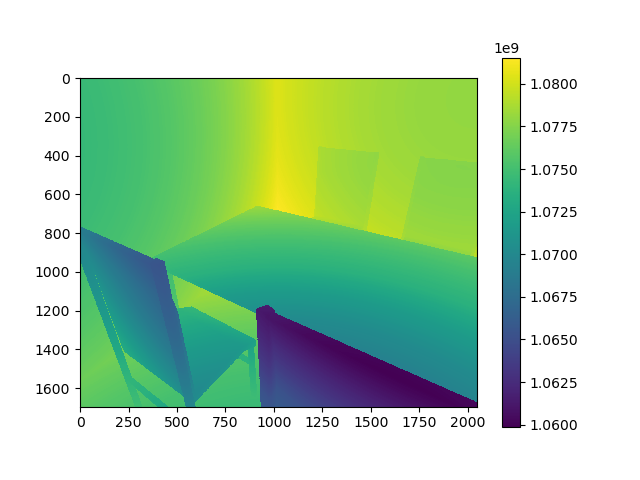
\includegraphics[width=0.32\textwidth]{img/ground-truth/1519695966968593.png}} 
    \subfigure{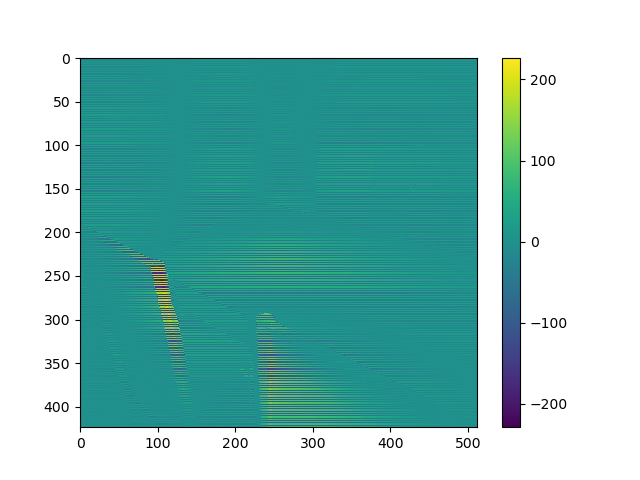
\includegraphics[width=0.32\textwidth]{img/deeptof-in/1519695966968593.png}} 
    \subfigure{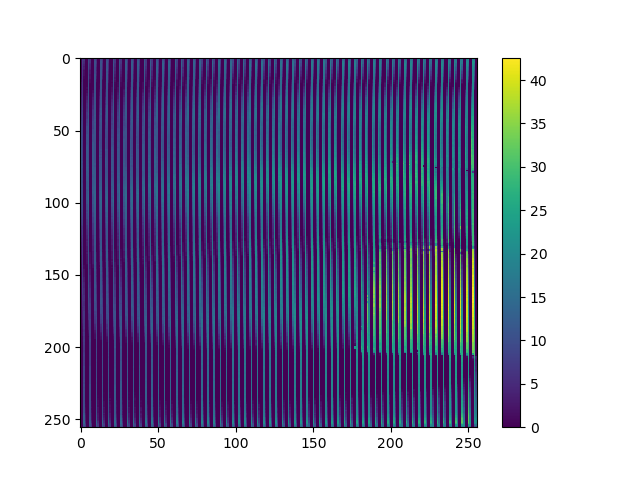
\includegraphics[width=0.32\textwidth]{img/deeptof-out/1519695966968593.png}}
    
    \subfigure{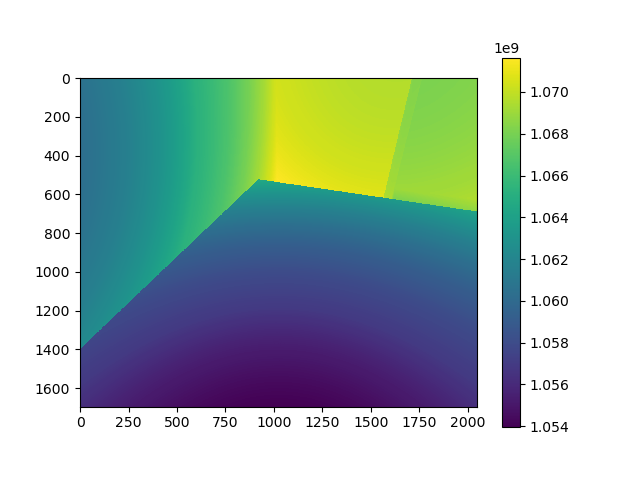
\includegraphics[width=0.32\textwidth]{img/ground-truth/1519748379130037.png}} 
    \subfigure{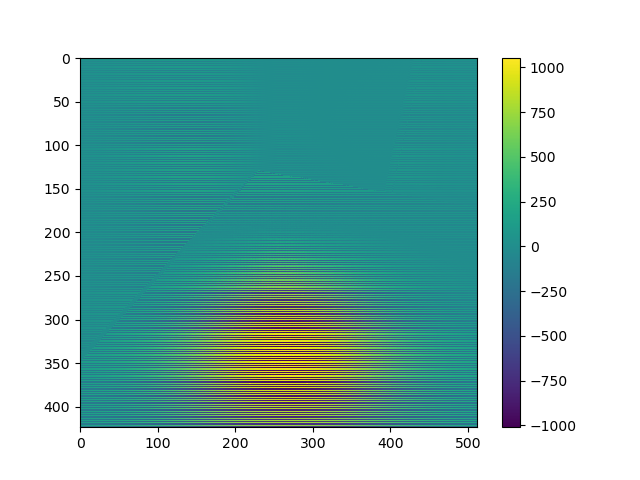
\includegraphics[width=0.32\textwidth]{img/deeptof-in/1519748379130037.png}} 
    \subfigure{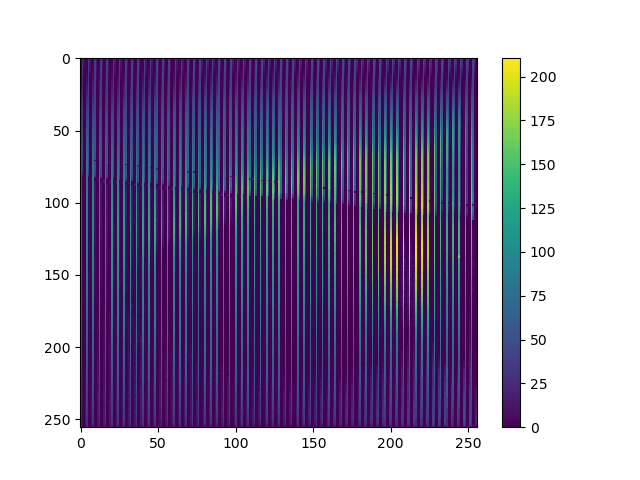
\includegraphics[width=0.32\textwidth]{img/deeptof-out/1519748379130037.png}} 
    
    \subfigure{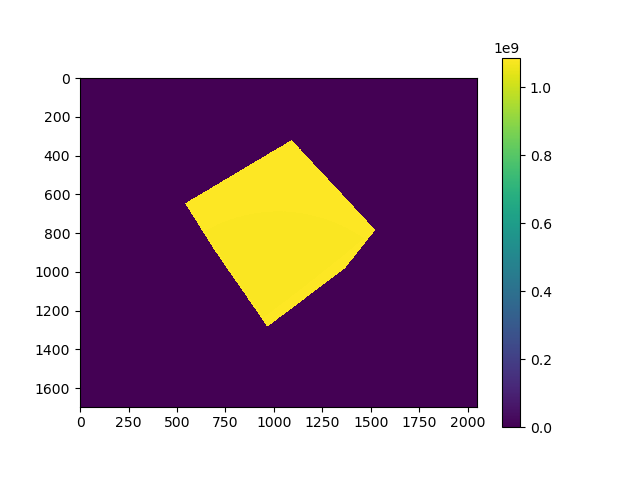
\includegraphics[width=0.32\textwidth]{img/ground-truth/1520215621311717.png}} 
    \subfigure{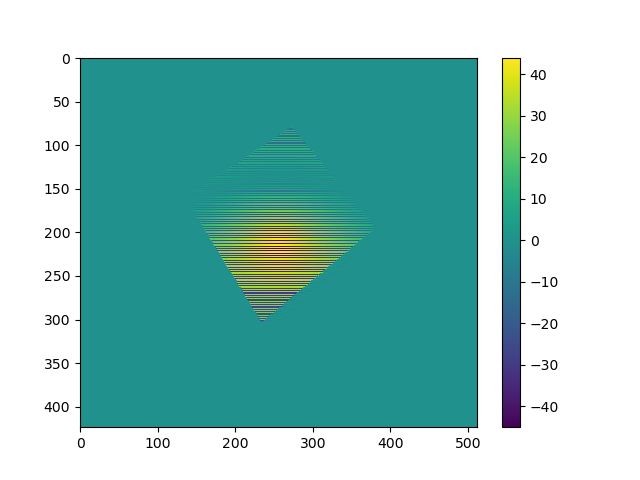
\includegraphics[width=0.32\textwidth]{img/deeptof-in/1520215621311717.png}} 
    \subfigure{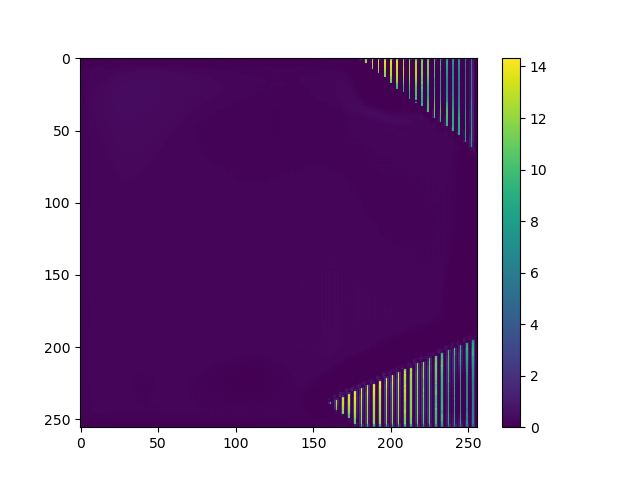
\includegraphics[width=0.32\textwidth]{img/deeptof-out/1520215621311717.png}}
    
    \subfigure{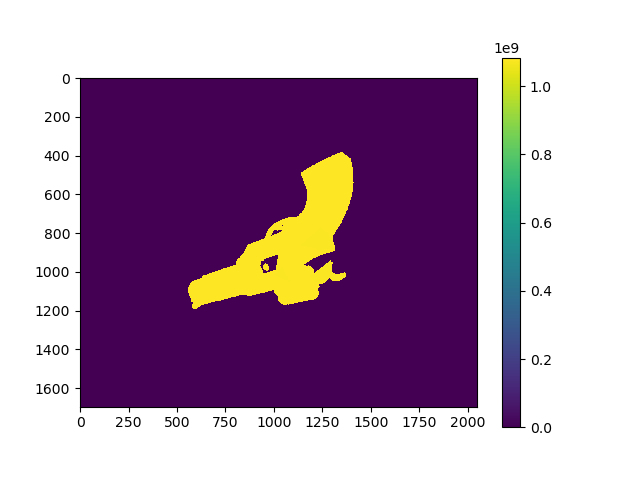
\includegraphics[width=0.32\textwidth]{img/ground-truth/1569126364657171.png}} 
    \subfigure{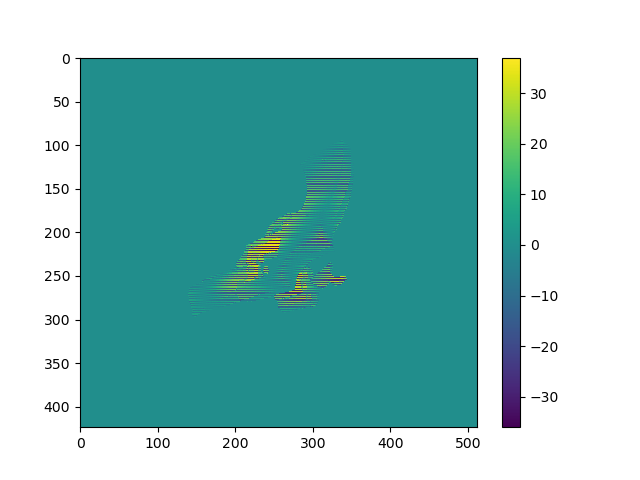
\includegraphics[width=0.32\textwidth]{img/deeptof-in/1569126364657171.png}} 
    \subfigure{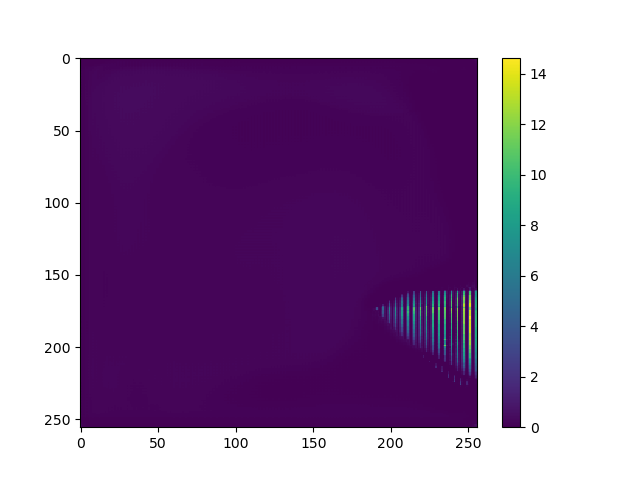
\includegraphics[width=0.32\textwidth]{img/deeptof-out/1569126364657171.png}}
    
    \subfigure{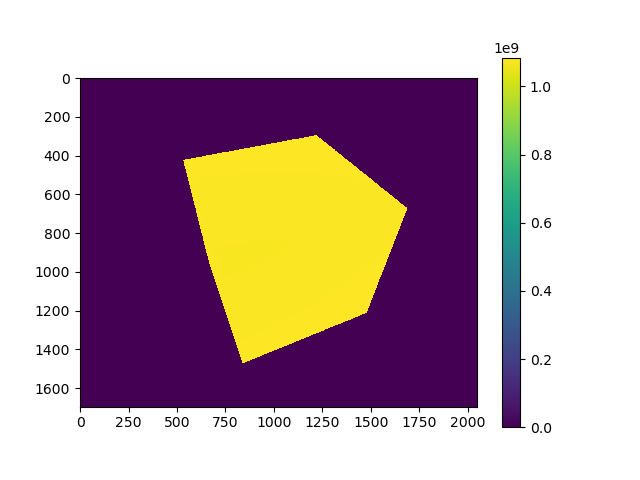
\includegraphics[width=0.32\textwidth]{img/ground-truth/1520215621721429.png}} 
    \subfigure{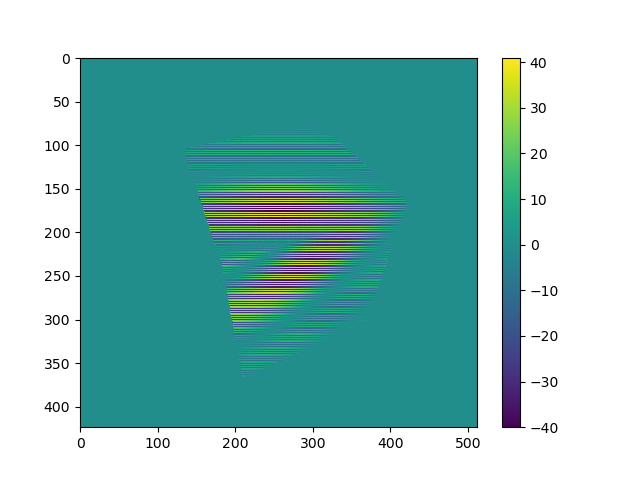
\includegraphics[width=0.32\textwidth]{img/deeptof-in/1520215621721429.png}} 
    \subfigure{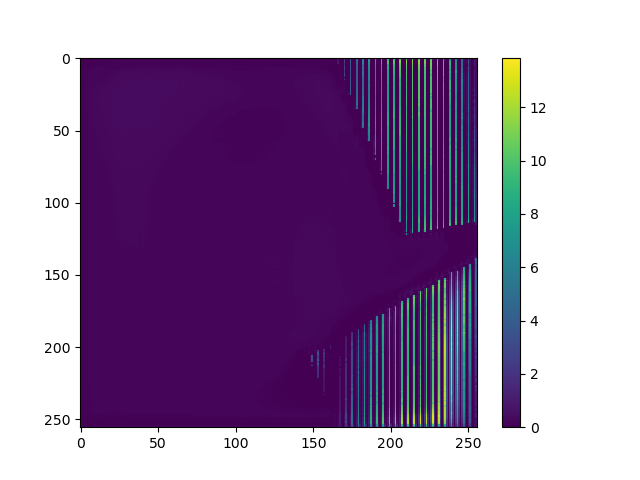
\includegraphics[width=0.32\textwidth]{img/deeptof-out/1520215621721429.png}}
    
    \caption{ . }
    \label{fig:deeptof_compare}
\end{figure}%
\end{comment}

\begin{figure}
    \centering
    \subfigure{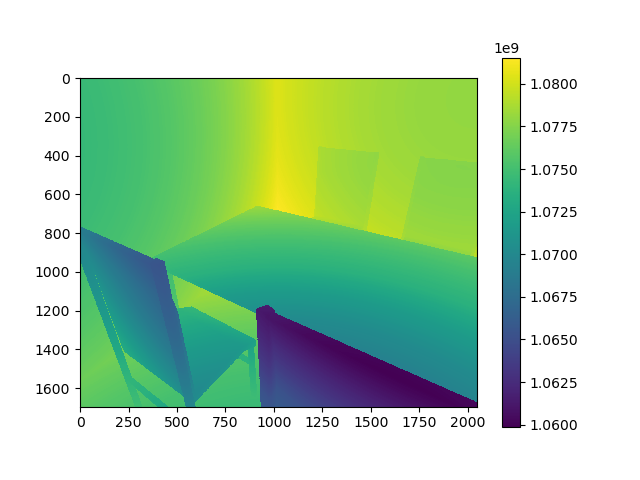
\includegraphics[width=25mm]{img/ground-truth/1519695966968593.png}}
    \subfigure{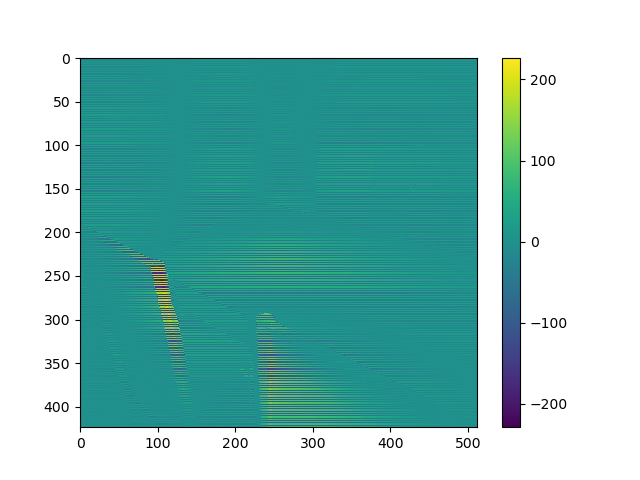
\includegraphics[width=25mm]{img/deeptof-in/1519695966968593.png}}
    \subfigure{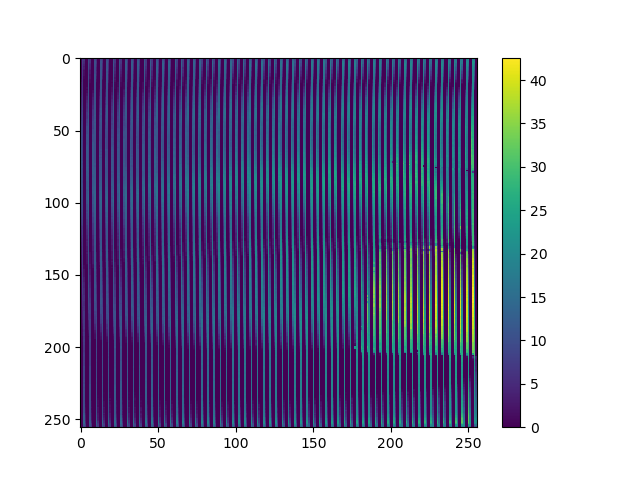
\includegraphics[width=25mm]{img/deeptof-out/1519695966968593.png}}
    \subfigure{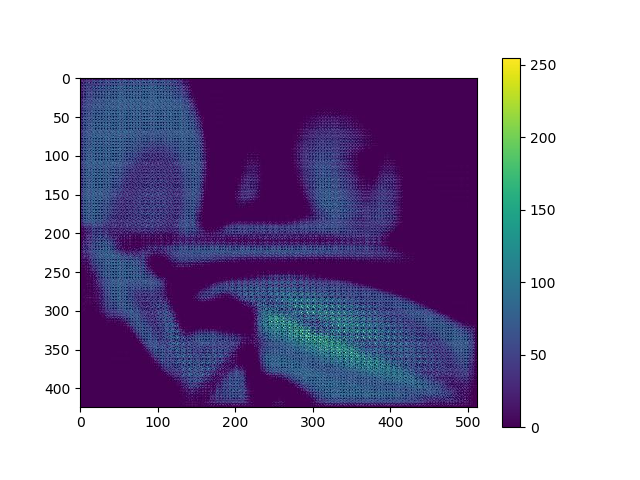
\includegraphics[width=25mm]{img/ours/Figure_1.png}}
    
    \subfigure{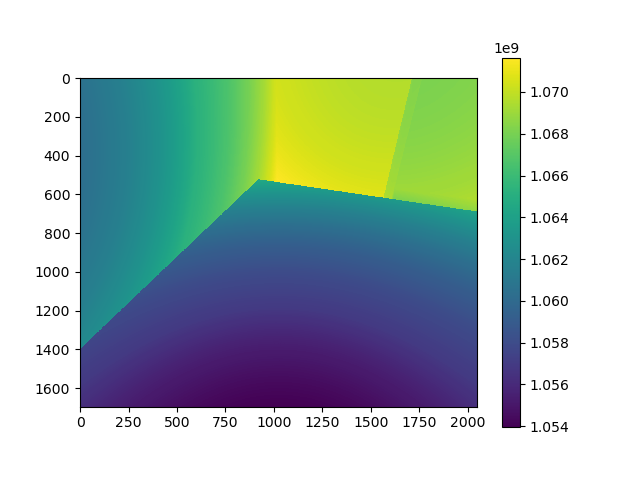
\includegraphics[width=25mm]{img/ground-truth/1519748379130037.png}}
    \subfigure{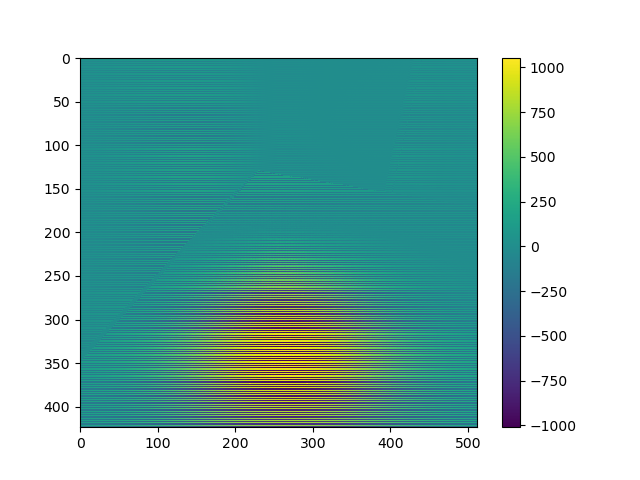
\includegraphics[width=25mm]{img/deeptof-in/1519748379130037.png}}
    \subfigure{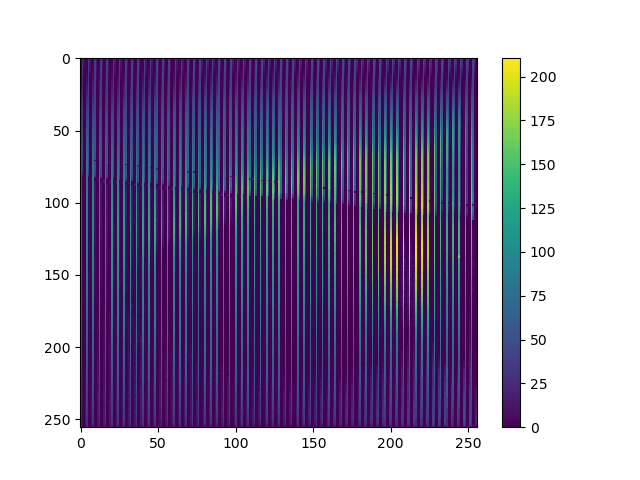
\includegraphics[width=25mm]{img/deeptof-out/1519748379130037.png}}
    \subfigure{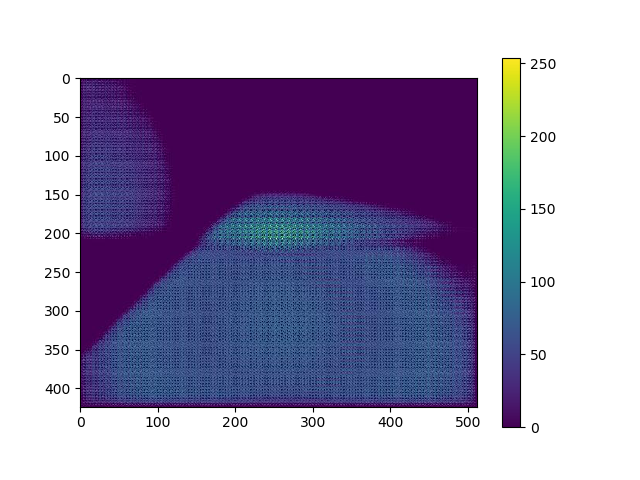
\includegraphics[width=25mm]{img/ours/Figure_2.png}}
    
    \subfigure{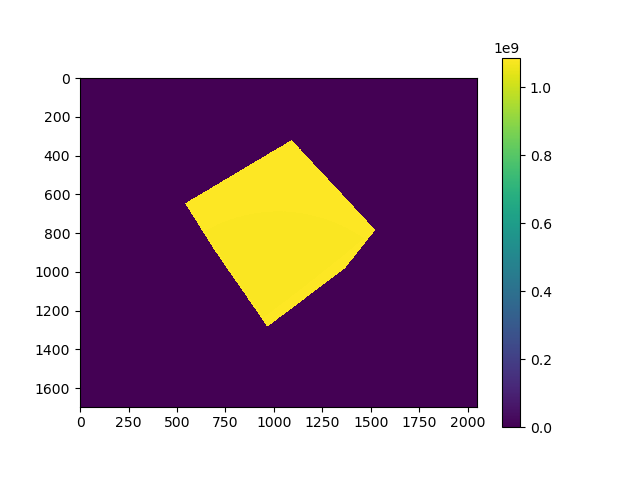
\includegraphics[width=25mm]{img/ground-truth/1520215621311717.png}}
    \subfigure{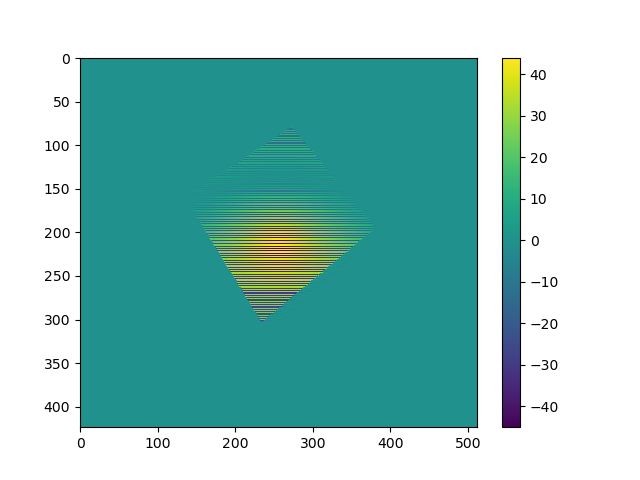
\includegraphics[width=25mm]{img/deeptof-in/1520215621311717.png}}
    \subfigure{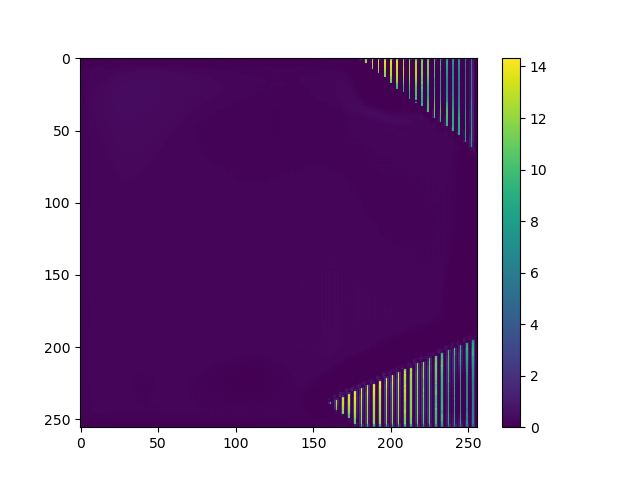
\includegraphics[width=25mm]{img/deeptof-out/1520215621311717.png}}
    \subfigure{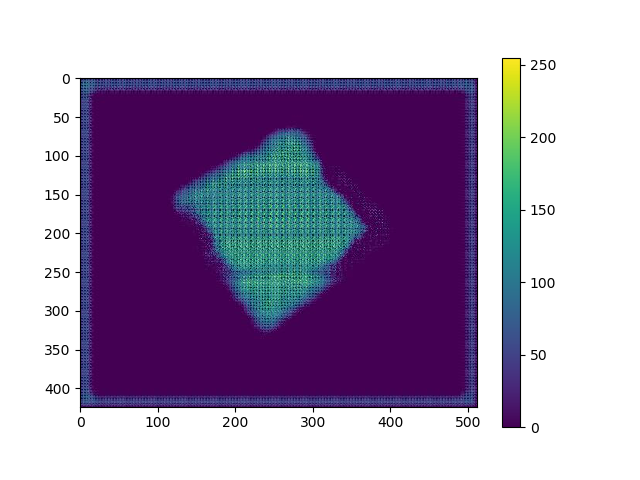
\includegraphics[width=25mm]{img/ours/Figure_3.png}}
    
    \subfigure{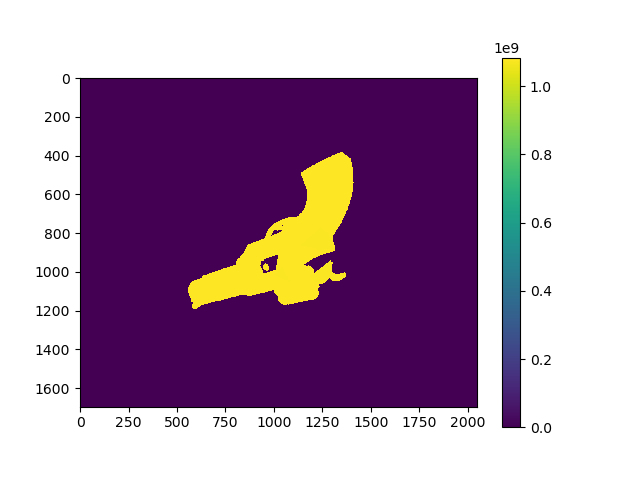
\includegraphics[width=25mm]{img/ground-truth/1569126364657171.png}}
    \subfigure{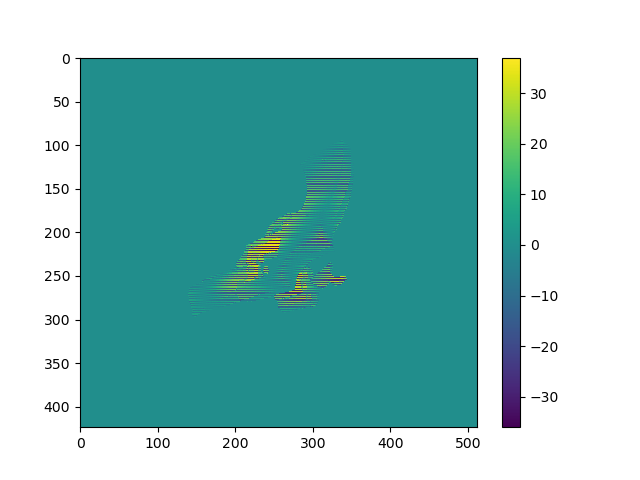
\includegraphics[width=25mm]{img/deeptof-in/1569126364657171.png}}
    \subfigure{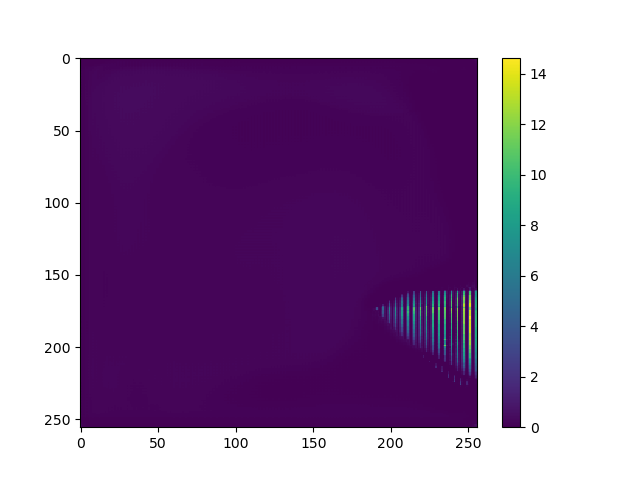
\includegraphics[width=25mm]{img/deeptof-out/1569126364657171.png}}
    \subfigure{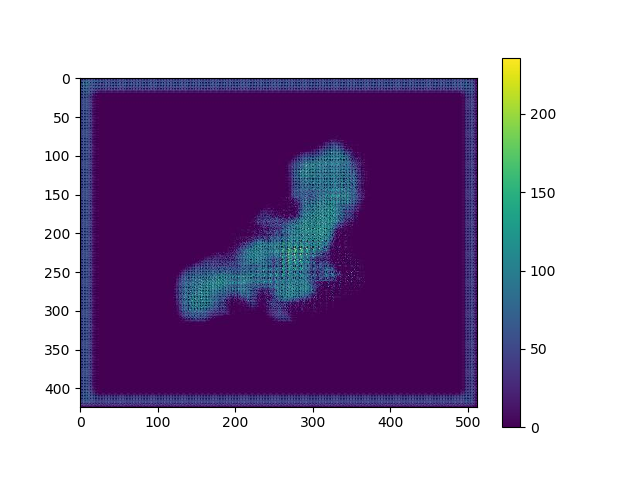
\includegraphics[width=25mm]{img/ours/Figure_4.png}}
    
    \subfigure[gt]{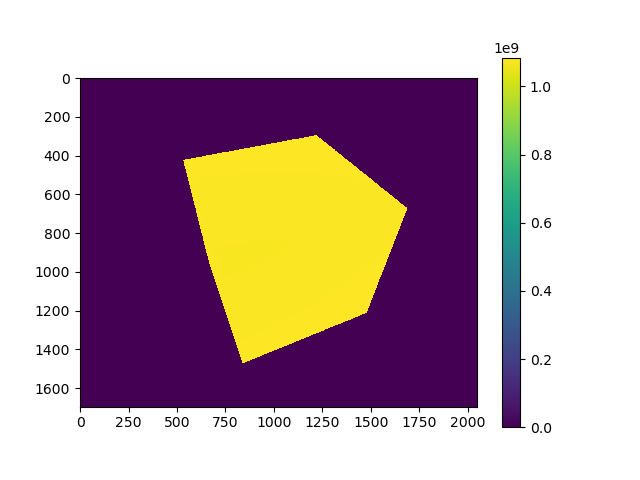
\includegraphics[width=25mm]{img/ground-truth/1520215621721429.png}}
    \subfigure[noisy]{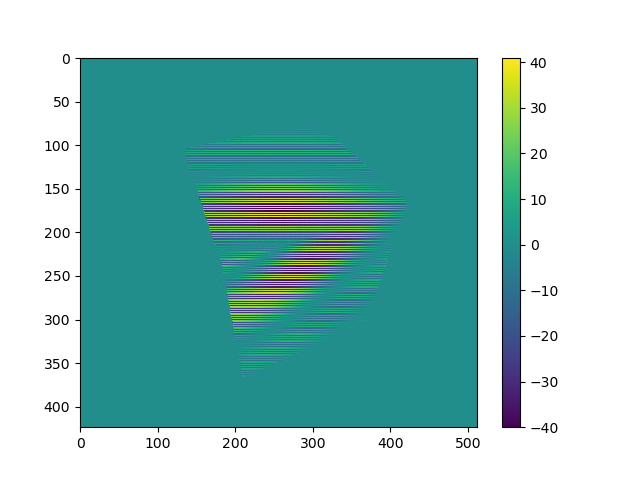
\includegraphics[width=25mm]{img/deeptof-in/1520215621721429.png}}
    \subfigure[DeepToF]{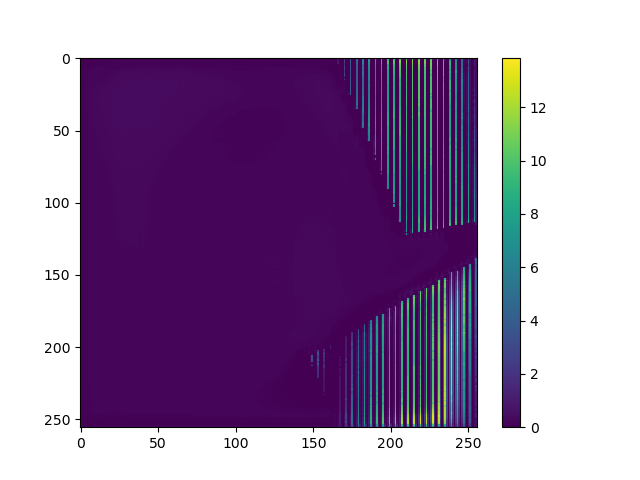
\includegraphics[width=25mm]{img/deeptof-out/1520215621721429.png}}
    \subfigure[\textbf{Ours}]{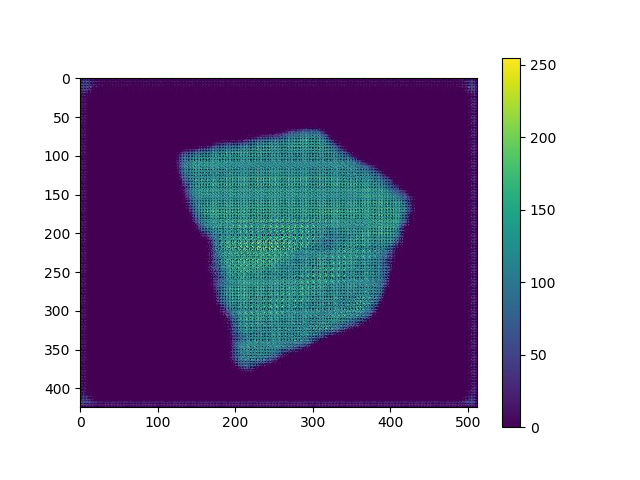
\includegraphics[width=25mm]{img/ours/Figure_5.png}}
    
    \caption{(a) Ground Truth images generated using simulator, (b) Kinect-based noisy images, (c) Output generated by DeepTof \cite{marco2017deeptof}, (d) Output generated by our method}
    \label{fig:deeptof_compare}
\end{figure}

%\lipsum[2-3]
The first model is able to correctly predict the scene parameters to the accuracy of 66.4\%, when the noise (Base Error) present in the data is 0.022050m. The second model is able to predict a True Depth Map using the parameters from the first model as input.
\newline
\newline
 We evaluated our model's output with respect to NVidia's general pipeline for denoising 3D ToF camera data. We also performed comparisons with DeepToF (See Figure \ref{fig:deeptof_compare}) and Phasor. We found that our model is able to perform better than Nvidia's Static Multi-Reflection Module (Static MRM).
    
    \begin{table}
    \centering
    \begin{tabular}{|c|c|c|c|}
    \hline
     & Median Depth Error & IQR of Depth Error & $90^{th}$ Percentile absolute error \\ \hline
    MRM & -0.01 & 2.63 & 4.19 \\ \hline
    DeepToF & -2.48 & 12.36 & 19.56 \\ \hline
    Phasor & -0.29 & 1.62 & 1.83 \\ \hline
        Ours & -0.38 & 4.89 & 21.15 \\ \hline
    
    \end{tabular}
    \caption{The table shows corresponding Median \& Inter-Quartile Range(IQR) Error of depth values, and 90th percentile of absolute error, in cm.}
    \label{tab:my-table}
\end{table}



% -----------------------------------------------------------------------
% Limitation
% -----------------------------------------------------------------------

\section{Limitations}

The model has been trained on a synthetic dataset. The performance on real-dataset is not as good as seen in testing because of the difference in noise statistics between real data and data simulated using the NVidia FLAT simulator. Since the model uses noise from the Kinect camera, results for Canesta camera's input depth maps are not of very high accuracy. 
\newline
\newline
We haven't included enough scenes with high specularity, and hence aren't able to handle objects present in a scene with high reflectance such as mirrors or metal surfaces. 

% -----------------------------------------------------------------------
% Conclusion
% -----------------------------------------------------------------------

\section{Conclusions}


Multi-Path Interference based noise is difficult to eliminate because it is difficult to model all possible light paths in a complex scene. We have introduced a novel technique that can be used to remove MPI based noise using a two-part deep learning network. We have shown that this method is able to predict the important scene parameters and outperform start-of-the-art methods in generating depth maps with lower errors. 


% \clearpage\mbox{}Page \thepage\ of the manuscript.
% \clearpage\mbox{}Page \thepage\ of the manuscript.
% \clearpage\mbox{}Page \thepage\ of the manuscript.
% \clearpage\mbox{}Page \thepage\ of the manuscript.
% \clearpage\mbox{}Page \thepage\ of the manuscript.
% \clearpage\mbox{}Page \thepage\ of the manuscript.
% \clearpage\mbox{}Page \thepage\ of the manuscript.
% This is the last page of the manuscript.
% \par\vfill\par
% Now we have reached the maximum size of the ECCV 2018 submission (excluding references).
% References should start immediately after the main text, but can continue on p.15 if needed.

%\clearpage

\bibliographystyle{splncs}
\bibliography{egbib}

\newpage
\appendix
% \addappheadtotoc
    
\section{Real-world data acquisition}

We used the Canesta D350 Time-of-Fligh camera to capture real-world depth-maps to go with the simulated dataset for training our network. The camera came with an EP Toolkit, but the company has since long discontinued support for the camera software. The toolkit only supports Windows XP Pro (32-bit) Operating System. We used Oracle's VirtualBox, a virtualization software that can emulate other operating systems in a sandbox environment. Luckily, we  found a Windows XP Pro ISO(installation) file online along with a product key. We also figured out how to share the virtual OS' filesystem with the host OS in order to collect data from the sandbox to local environment. 

We have collected 50 images using objects with varying lambertian reflectance such as whiteboards, water bottles, microwave oven etc. The depth maps captured by the camera are (64x64) images with heat-maps for distance visualization.

\section{Remote Server Setup}

Since we did not have enough compute resources to generate data or run the model from NVLabs' software, we tried a few different options such as Google Colab, Google Cloud \& AWS and finally settled on the Nautilus Hypercluster. Google Colab has a 12-hour state, \& it dumps all work on Google Drive and removes previous state after that 12hr window is done. Google Cloud and AWS are paid software that we had difficult time understanding the working of as well as the method of sharing same instance with each other.

Nautilus Hypercluster uses the Kubernetes container orchestration software to manage Docker Images. We used a stateful data storage job (using Ceph) as our storage space for the dataset. We edited over Pytorch's docker image to install required software for running various other software such as the transient renderer, deeptof for comparison, and text editor, screen, opencv etc. We had to go over multiple iterations of setup because of the complicated nature of setting up a Job(long-running , stateful) and a Pod(6-hr state) on Kubernetes. We also had to learn a few softwares like screen (for working on multiple terminals in parallel), rsync(intelligent data downloader) and vim(text editor) to work on a remote server. We had little experience working with Docker and no experience with Kubernetes, so it took a lot of time for us to use the platform for all required tasks.

The code for our work on deploying Jobs \& Pods to Kubernetes and Docker Images to Hub is present at
\href{https://www.github.com/daemonslayer/kubernetes.git}{\textbf{github.com/daemonslayer/kubernetes.git}} where we have added details on how to use the server.

%Due to the size of the NVlabs FLAT dataset (576GB), we are unable to use the simulator locally on our machines.%
%Thus we have successfully deployed the FLAT simulator on the Nautilus Hyper Cluster and using Kubernetes (similar to Docker) for managing the applications. %

%Typical Pods in Kubernetes only exist for at most 6 hours, thus it is incapable of performing any training tasks. However, We have managed to migrate the application and the dataset to a persistent storage Pod; this enables us to continue our research and save the progress. We create Jobs and Pods for the purpose of experimenting, training, and evaluating our model on the cloud.%

\section{Transient Renderer Setup}

We setup the transient renderer and generated a few scenes. These scenes can be used to generate noisy depth map images using NVLabs' FLAT simulation tool.

\section{Data Generation Tool by NVLabs}

The FLAT simulator consists of 1027 scene images rendered using transient rendered with different meshes, lighting, and lambertian reflectance properties. The simulator also has Kinect Camera Function, a function that stores how much incident light is modulated by the camera to calculate the depth information. The dataset also has 2000 noise samples for a kinect camera to generate varying noisy depth maps from rendered ground-truth images. 

We generated 1027 noisy and ground-truth imags using the FLAT dataset. Since the dataset takes about 7-8 minutes per image per noise type (since they deal with 4 different noises), and has high RAM requirement, we first went through the code to only generate MPI-noise images and tried to parallelize the code using python's multiprocessing library. The method of first converting a rendered image into a depth map and then adding noise to it is a bit unintuitively presented in the code. This led to a lot of time being spent in experimenting with the tool to create the data that we needed.

\section{Various Experiments on Data}

We experimented with multiple deep-learning models as well as different loss functions.  

\section{Running Models for Comparison}

We have compared our work with two previous works, DeepToF and MRM. We also tried making Phasor work but the has been written in MatLab and has high compute requirement. We tried using an Octave docker image to run it on the server, but weren't successful.

DeepToF has been written in Caffe Deep-Learning Library. We tried to install caffe in our local machine, but there were too many bugs and issues in the process. After a few iterations, we found a working Docker Image that we edited to get the required Caffe(with GPU support) environment running. Since Caffe has a not-so-transparent documentation, it took us some time to get the model running and producing outputs.

MRM: The MRM model from NVidia had some bugs in the code due to the authors not having uploaded all their data and instead leaving it to the user to generate as required. The code also used deprecated packages such as scipy which weren't working with new version. We replaced the code and made some other changes as required to make the code work. 
\end{document}
